\documentclass[a4paper,11pt,landscape,exos]{nsi} % COMPILE WITH DRAFT
\usepackage{hyperref}

\pagestyle{empty}
\setlength{\columnseprule}{0.5pt}
\setlength{\columnsep}{1cm}
\begin{document}

\begin{multicols}{2}
\classe{\premiere spe}
\titre{
\includegraphics[width=3cm]{CAN.png} Entrainement 4}
\maketitle

\begin{enumerate}[]
	\item $0{,}8\times6$
	\item Affirmation : \\
    Le point $A(-1\,;\,5)$ appartient à la parabole d'équation $y=x^2+5$ \\	$\square\;$ Vrai \qquad $\square\;$ Faux\qquad 
	\item Développer et réduire l'expression $(x+3)(x+4)$.
	\item $3+\dfrac{4}{3}$ 
	\item $10\,\%$ de $20$
	\item Médiane de la série : $\quad 20\,;\,12\,;\,10\,;\,15\,;\,7$
	\item Multiplier une quantité par $0{,}95$ revient à la diminuer de : $\ldots\,\%$
	\item $(u_n)$ est une suite géométrique telle que $u_0=3$ et $u_1=-21$\\La raison de cette suite est :  $\ldots$
	\item Compléter par deux entiers consécutifs : $\ldots < \sqrt{74} < \ldots$
	\item Solution de l'équation $7x+4=8$
	\item  Factoriser   $-4(2x-5)+(2x-5)^2$.
	\item Dans une base orthonormée : $\vc{u}{-2}{1}$ et  $\vc{v}{4}{-2}$.\\
    Alors $\vec{u}$ et $\vec{v}$ sont colinéaires.\\	$\square\;$ Vrai \qquad $\square\;$ Faux\qquad
	\item Déterminer l'équation réduite de la droite $(AB)$.\\    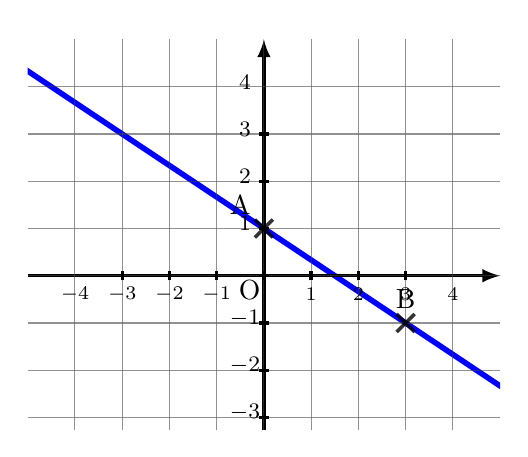
\begin{tikzpicture}[baseline,scale = 0.6]

    \tikzset{
      point/.style={
        thick,
        draw,
        cross out,
        inner sep=0pt,
        minimum width=5pt,
        minimum height=5pt,
      },
    }
    \clip (-5,-3.25) rectangle (5,5.25);
    	\draw [color={black}] (-0.3,-0.3) node[anchor = center,scale=1, rotate = 0] {O};
	\draw[color={blue},line width = 2] (-41.55,28.7)--(44.55,-28.7);
	\draw[color ={black},line width = 1.2,>=latex,->] (-5,0)--(5,0);
	\draw[color ={black},line width = 1.2,>=latex,->] (0,-4)--(0,5);
	\draw[color ={black},opacity = 0.4] (-5,1)--(5,1);
	\draw[color ={black},opacity = 0.4] (-5,-1)--(5,-1);
	\draw[color ={black},opacity = 0.4] (-5,2)--(5,2);
	\draw[color ={black},opacity = 0.4] (-5,-2)--(5,-2);
	\draw[color ={black},opacity = 0.4] (-5,3)--(5,3);
	\draw[color ={black},opacity = 0.4] (-5,-3)--(5,-3);
	\draw[color ={black},opacity = 0.4] (-5,4)--(5,4);
	\draw[color ={black},opacity = 0.4] (-5,-4)--(5,-4);
	\draw[color ={black},opacity = 0.4] (1,-4)--(1,5);
	\draw[color ={black},opacity = 0.4] (-1,-4)--(-1,5);
	\draw[color ={black},opacity = 0.4] (2,-4)--(2,5);
	\draw[color ={black},opacity = 0.4] (-2,-4)--(-2,5);
	\draw[color ={black},opacity = 0.4] (3,-4)--(3,5);
	\draw[color ={black},opacity = 0.4] (-3,-4)--(-3,5);
	\draw[color ={black},opacity = 0.4] (4,-4)--(4,5);
	\draw[color ={black},opacity = 0.4] (-4,-4)--(-4,5);
	\draw[color ={gray},opacity = 0.3] (-5,0)--(5,0);
	\draw[color ={gray},opacity = 0.3] (-5,1)--(5,1);
	\draw[color ={gray},opacity = 0.3] (-5,-1)--(5,-1);
	\draw[color ={gray},opacity = 0.3] (-5,2)--(5,2);
	\draw[color ={gray},opacity = 0.3] (-5,-2)--(5,-2);
	\draw[color ={gray},opacity = 0.3] (-5,3)--(5,3);
	\draw[color ={gray},opacity = 0.3] (-5,-3)--(5,-3);
	\draw[color ={gray},opacity = 0.3] (-5,4)--(5,4);
	\draw[color ={gray},opacity = 0.3] (-5,-4)--(5,-4);
	\draw[color ={gray},opacity = 0.3] (0,-4)--(0,5);
	\draw[color ={gray},opacity = 0.3] (1,-4)--(1,5);
	\draw[color ={gray},opacity = 0.3] (-1,-4)--(-1,5);
	\draw[color ={gray},opacity = 0.3] (2,-4)--(2,5);
	\draw[color ={gray},opacity = 0.3] (-2,-4)--(-2,5);
	\draw[color ={gray},opacity = 0.3] (3,-4)--(3,5);
	\draw[color ={gray},opacity = 0.3] (-3,-4)--(-3,5);
	\draw[color ={gray},opacity = 0.3] (4,-4)--(4,5);
	\draw[color ={gray},opacity = 0.3] (-4,-4)--(-4,5);
	\draw[color ={black},line width = 1.2] (0,-0.1)--(0,0.1);
	\draw[color ={black},line width = 1.2] (1,-0.1)--(1,0.1);
	\draw[color ={black},line width = 1.2] (-1,-0.1)--(-1,0.1);
	\draw[color ={black},line width = 1.2] (2,-0.1)--(2,0.1);
	\draw[color ={black},line width = 1.2] (-2,-0.1)--(-2,0.1);
	\draw[color ={black},line width = 1.2] (3,-0.1)--(3,0.1);
	\draw[color ={black},line width = 1.2] (-3,-0.1)--(-3,0.1);
	\draw[color ={black},line width = 1.2] (-0.1,0)--(0.1,0);
	\draw[color ={black},line width = 1.2] (-0.1,1)--(0.1,1);
	\draw[color ={black},line width = 1.2] (-0.1,-1)--(0.1,-1);
	\draw[color ={black},line width = 1.2] (-0.1,2)--(0.1,2);
	\draw[color ={black},line width = 1.2] (-0.1,-2)--(0.1,-2);
	\draw[color ={black},line width = 1.2] (-0.1,3)--(0.1,3);
	\draw[color ={black},line width = 1.2] (-0.1,-3)--(0.1,-3);
	\draw (1,-0.4) node[anchor = center, rotate=0] {\scriptsize \color{black}{$1$}};
	\draw (2,-0.4) node[anchor = center, rotate=0] {\scriptsize \color{black}{$2$}};
	\draw (3,-0.4) node[anchor = center, rotate=0] {\scriptsize \color{black}{$3$}};
	\draw (4,-0.4) node[anchor = center, rotate=0] {\scriptsize \color{black}{$4$}};
	\draw (-1,-0.4) node[anchor = center, rotate=0] {\scriptsize \color{black}{$-1$}};
	\draw (-2,-0.4) node[anchor = center, rotate=0] {\scriptsize \color{black}{$-2$}};
	\draw (-3,-0.4) node[anchor = center, rotate=0] {\scriptsize \color{black}{$-3$}};
	\draw (-4,-0.4) node[anchor = center, rotate=0] {\scriptsize \color{black}{$-4$}};
	\draw (-0.4,1.1) node[anchor = center, rotate=0] {\footnotesize \color{black}{$1$}};
	\draw (-0.4,2.1) node[anchor = center, rotate=0] {\footnotesize \color{black}{$2$}};
	\draw (-0.4,3.1) node[anchor = center, rotate=0] {\footnotesize \color{black}{$3$}};
	\draw (-0.4,4.1) node[anchor = center, rotate=0] {\footnotesize \color{black}{$4$}};
	\draw (-0.4,-0.9) node[anchor = center, rotate=0] {\footnotesize \color{black}{$-1$}};
	\draw (-0.4,-1.9) node[anchor = center, rotate=0] {\footnotesize \color{black}{$-2$}};
	\draw (-0.4,-2.9) node[anchor = center, rotate=0] {\footnotesize \color{black}{$-3$}};
	\draw[color ={black},line width = 1.25,opacity = 0.8] (2.81,-0.81)--(3.19,-1.19);\draw[color ={black},line width = 1.25,opacity = 0.8] (2.81,-1.19)--(3.19,-0.81);
	\draw[color ={black},line width = 1.25,opacity = 0.8] (-0.19,1.19)--(0.19,0.81);\draw[color ={black},line width = 1.25,opacity = 0.8] (-0.19,0.81)--(0.19,1.19);
	\draw [color={black}] (-0.5,1.5) node[anchor = center,scale=1, rotate = 0] {A};
	\draw [color={black}] (3,-0.5) node[anchor = center,scale=1, rotate = 0] {B};

\end{tikzpicture}\\
	\item Soit la suite $(u_n)$ définie  par $u_0 = 1$ et pour $n \in \mathbb{N}$, 
    $u_{n+1} = 3u_n +1$.\\
    $u_2=$ $\ldots$
	\item $P(A\cap B)=0{,}24$ ; $\quad P(A)=0{,}4\,\,; \quad P(B)=0{,}6$\\$A$ et $B$ sont indépendants.\\	$\square\;$ Vrai\qquad $\square\;$ Faux\qquad 
	\item Le discriminant du trinôme $x^2+x-2$ est  $\ldots$
	\item Un sportif court $3\,500$ m  en $15$ min.\\
      Quelle est sa vitesse en km/h ?
	\item $f(x)=x^2-2x-6\ ; \qquad$
    $f'(x)=$ $\ldots$
	\item $\renewcommand{\arraystretch}{1}
\begin{array}{|c|c|c|c|c|}
\hline
\cellcolor{lightgray} x_i & \cellcolor{lightgray} 0 & \cellcolor{lightgray} 1 & \cellcolor{lightgray} \,\,\,\,2\,\,\,\, & \cellcolor{lightgray} \,\,\,\,3\,\,\,\,\\
\hline
 \rule[-2ex]{0pt} {6ex}\ \cellcolor{lightgray} P(X=x_i) & 0{,}25 & 0{,}05 & 0{,}5 & \ldots\\
\hline
 \end{array}
\renewcommand{\arraystretch}{1}$


\medskip
 $P(X=3)=$ $\ldots$
	\item $f(x)=\dfrac{1}{x^3}\ ;\qquad$
    $f'(x)=$ $\ldots$
	\item Solutions de $(x-6)(x-4)  < 0$
	\item Soit $f\,:\,x\longmapsto (x+7)(x+1) $\\
    La représentation graphique $\mathcal{C}_f$ a pour axe de symétrie la droite d’équation :	$\quad x=\ldots$
	\item $\dfrac{2^4}{2^7}=2^{\ldots}$
	\item Écrire sous la forme d'une fraction irréductible :
          $\quad \dfrac{3}{4} + \dfrac{5}{6}=$
              $\ldots$
	\item On donne l'arbre de probabilités ci-dessous :\\
    \def\abun{A}
 \def\alun{0,7}
 \def\abdeux{$\barmaj{A}$}
 \def\aldeux{}
 \def\abtrois{$B$}
 \def\altrois{0,2}
 \def\abquatre{$\barmaj{B}$}
 \def\alquatre{}
\def\abcinq{$B$}
 \def\alcinq{0,5}
 \def\absix{$\barmaj{B}$}
 \def\alsix{}
 %\begin{center}
 \arbreproba\\
 %\end{center}
    $P(B)=\ldots$ 

	\item Augmenter un prix de $16\,\%$ puis le  diminuer de $50\,\%$ revient à le
    diminuer de $50\,\%$  puis à l’augmenter $16\,\%$.\\	$\square\;$ Vrai \qquad $\square\;$ Faux\qquad 
	\item Soit $f(x)=-x^2-8x+1$\\
    L'abscisse du sommet de la parabole qui représente $f$ est : $\ldots$

    \item Calculer $2\,025^2-2\,024^2$.
    \item Coordonnées du point $M$ milieu du segment $[AB]$ où $A(10\,;\,2)$ et $B(8\,;\,10)$
    
	\item  Factoriser  $x^2-100$.
\end{enumerate}
\vfill\null
\columnbreak
NOM, Prénom :  \\

Score : \ldots\ldots / 30
\end{multicols}

\newpage

\begin{multicols}{2}
    \classe{\premiere spe}
\titre{
\includegraphics[width=3cm]{CAN.png} Corrigé 4}
\maketitle

\begin{enumerate}[]

    \item On peut calculer ainsi : \\
    $\begin{aligned}
    0{,}8\times6&=0,1\times 8\times6\\
    &=0,1\times 48\\
    &={\color[HTML]{f15929}\boldsymbol{4{,}8}}
    \end{aligned}$
\item Le point $A$ est sur la parabole si son ordonnée est égale à l'image de son abscisse. \\
    $\begin{aligned}
        f(-1)&=(-1)^2+5\\
        &=6
        \end{aligned}$
        \\
        Puisque $6 \neq 5$, le point $A$ n'est pas sur la parabole. \\L'affirmation est {\bfseries \color[HTML]{f15929}FAUSSE}
\item $\begin{aligned}
      (x+3)(x+4)&=x^2+4x+3x+12\\
      &={\color[HTML]{f15929}\boldsymbol{x^2+7x+12}}
      \end{aligned}$\\Le terme en $x^2$ vient de $x\times 1x=x^2$.\\Le terme en $x$ vient de la somme de $x \times 4$ et de $3 \times 1x$.\\Le terme constant vient de $3\times 4= 12$.
\item $\begin{aligned}
      3+\dfrac{4}{3} &= \dfrac{3 \times 3}{3} + \dfrac{4}{3} \\
      &= \dfrac{9}{3} + \dfrac{4}{3}\\
      &  ={\color[HTML]{f15929}\boldsymbol{\dfrac{13}{3}}}
      \end{aligned}$
\item $10\,\%$ de $20 = 0,1 \times 20={\color[HTML]{f15929}\boldsymbol{2}}$\\ Prendre $10\,\%$  d'une quantité revient à la diviser par $10$.\\
      Ainsi, $10\,\%$ de $20 = \dfrac{20}{10}=2$.
\item Cette série comporte cinq valeurs, on les range dans l'ordre croissant :\\
      $7\,;\,10\,;\,12\,;\,15\,;\,20$\\
      La médiane est la valeur centrale, soit ${\color[HTML]{f15929}\boldsymbol{12}}$.

\item Comme $0{,}95-1=-0{,}05$, multiplier par $0{,}95$ revient à diminuer de ${\color[HTML]{f15929}\boldsymbol{5}}\,\%$. 
\item La raison de la suite est donnée par le quotient $\dfrac{u_1}{u_0}=\dfrac{-21}{3}={\color[HTML]{f15929}\boldsymbol{-7}}$.
\item Comme $64 < 74 < 81$, alors 
    ${\color[HTML]{f15929}\boldsymbol{8}} < \sqrt{74} < {\color[HTML]{f15929}\boldsymbol{9}}$.
\item On procède par étapes successives :\\
      On commence par isoler $7x$ dans le membre de gauche en retranchant
      $4$ dans chacun des membres, puis on divise
      par $7$ pour obtenir la solution : \\
       $\begin{aligned}
       7x+4&=8\\
      7x&=8-4\\
      7x&=4\\
      x&=\dfrac{4}{7}    
      \end{aligned}$\\
      La solution de l'équation est : ${\color[HTML]{f15929}\boldsymbol{\dfrac{4}{7}}}$.
      
\item $(2x-5)$ est un facteur commun.\\
      $\begin{aligned}
      -4(2x-5)+(2x-5)^2
      &=(2x-5)(-4+(2x-5))\\
      &={\color[HTML]{f15929}\boldsymbol{(2x-5)(2x-9)}}\end{aligned}$
\item  Les vecteurs non nuls $\vec{u}$ et $\vec{v}$ sont colinéaires si et seulement si il existe un nombre $k$ tel que $\vec{v}=k\vec{u}$.\\
    Les coordonnées de $\vec{v}$ sont égales à $-2$ fois celles de $\vec{u}$.\\
    Donc $\vec{v}=-2\vec{u}$ et les vecteurs $\vec{u}$ et $\vec{v}$ sont colinéaires.\\
    L'affirmation est {\bfseries \color[HTML]{f15929}VRAIE}.
\item En utilisant les deux points $A$ et $B$, on détermine le coefficient directeur $m$ de la droite : \\
    $m=\dfrac{y_B-y_A}{x_B-x_A}=-\dfrac{2}{3}$.\\
         L' ordonnée à l'origine est $1$, ainsi l'équation réduite de la droite est ${\color[HTML]{f15929}\boldsymbol{y=-\dfrac{2}{3}x+1}}$.

\item On calcule d'abord $u_1$ : \\   
      $\begin{aligned}
      u_1&=3\times u_0 +1\\
      u_1&=3\times 1 +1\\
      &=4     
      \end{aligned}$\\
      On obtient donc pour $u_2$ :\\
      $\begin{aligned}
      u_2&=3\times u_1 +1\\
      u_2&=3\times 4 +1\\
      &={\color[HTML]{f15929}\boldsymbol{13}}     
      \end{aligned}$
\item $A$ et $B$ sont indépendants si $P(A\cap B)=P(A)\times P(B)$.\\
    Comme :\\$\begin{aligned}
    P(A)\times P(B)&=0{,}4\times 0{,}6\\
    &=0{,}24
    \end{aligned}$\\On obtient l'égalité  $P(A\cap B)=P(A)\times P(B)$.\\
    Les événements $A$ et $B$ sont donc indépendants.\\ L'affirmation est {\bfseries \color[HTML]{f15929}VraiE}.
\item  $\Delta=b^2-4ac$ avec $a=1$, $b=1$ et $c=-2$.\\
      $\begin{aligned}
      \Delta&=1^2-4\times 1\times (-2) \\
      &={\color[HTML]{f15929}\boldsymbol{9}} 
      \end{aligned}$
\item En $1$ heure, il parcourt $4$ fois plus de distance  qu'en $15$ minutes, soit $4\times 3\,500=
      14\,000$ m.\\
      Sa vitesse est donc ${\color[HTML]{f15929}\boldsymbol{14}}$ km/h.
\item  On détermine la fonction dérivée :\\
      $\begin{aligned}
      f'(x)&= 2x -2\times 1 +0\\
      &={\color[HTML]{f15929}\boldsymbol{2x-2}}     
      \end{aligned}$
\item  On calcule l'espérance mathématiques de $X$ : \\
    $\begin{aligned}
      P(X=3) &=1-(0,25+0,05+0,5)\\
      &=1-0,8\\
      &={\color[HTML]{f15929}\boldsymbol{0,2}}
      \end{aligned}$
      
\item  
    $\begin{aligned}
  f'(x)&=\dfrac{-3}{x^{3+1}}\\
  &={\color[HTML]{f15929}\boldsymbol{-\dfrac{3}{x^4}}}
  \end{aligned}$
\item $(x-6)(x-4)$ est l'expression factorisée d'une fonction polynôme du second degré de la forme $a(x-x_1)(x-x_2)$.\\
    Les racines sont $x_1=6$ et $x_2=4$. \\
    Le polynôme est du signe de $a=1$ (donc positif) sauf entre ses racines.\\
    L'ensemble solution est donc :  ${\color[HTML]{f15929}\boldsymbol{]4\,;\,6[}}$.   
     
\item Les racines de ce polynôme du second degré sont $x_1=-7$ et $x_2=-1$.\\
    L'axe de symétrie est donné par la moyenne des racines : $x=\dfrac{x_1+x_2}{2}$, soit $x=\dfrac{-7+(-1)}{2}$, c'est-à-dire ${\color[HTML]{f15929}\boldsymbol{x=-4}}$.
\item $\dfrac{2^4}{2^7}=2^{4-7}=2^{\color[HTML]{f15929}\boldsymbol{-3}}$

\item Pour additionner des fractions, on les met au même dénominateur.\\
  Le plus petit dénominateur commun est $12$.\\
             Ainsi, \\
           $\begin{aligned}
           \dfrac{3}{4} + \dfrac{5}{6}&=
            \dfrac{9}{12}+\dfrac{10}{12} \\
           &={\color[HTML]{f15929}\boldsymbol{\dfrac{19}{12}}}\text{(fraction irréductible)}
           \end{aligned}$
             
             
            
\item On utilise la formule des probabilités totales pour calculer $P(B)$ :\\
          $\begin{aligned}
          P(B)&=P(A\cap B)+P(\bar{A}\cap B)\\
          &=0{,}7\times 0{,}2+0{,}3\times 0{,}5\\
            &=0{,}14+0{,}15\\
&={\color[HTML]{f15929}\boldsymbol{0{,}29}}
          \end{aligned}$
      
\item Le coefficient multiplicateur global est le produit des coefficients multiplicateurs.\\
    Le coefficient multiplicateur associé à une augmentation de $16\,\%$ est $1{,}16$ et celui associé à une diminution de 
    $50\,\%$ est $0{,}5$.\\ 
    Le coefficient multiplicateur gobal est  $1{,}16\times 0{,}5$ dans un cas ou $0{,}5\times 1{,}16$ dans l'autre cas, ce qui revient strictement au même. 
    \\
  L'affirmation est donc  {\bfseries \color[HTML]{f15929}VraiE}.
\item Pour un polynôme de degré $2$ du type $ax^2+bx+c$, l'abscisse du sommet 
    de la parabole $x_S$ est donnée par $-\dfrac{b}{2a}$.\\
     L'abscisse du sommet est donnée  par $x_S=-\dfrac{-8}{2\times (-1)}={\color[HTML]{f15929}\boldsymbol{-4}}$.
     
   


 \item On utilise l'égalité remarquable $a^2-b^2=(a-b)(a+b)$ avec $a=2\,025$ et $b=2\,024$.\\
        $2\,025^2-2\,024^2=(2\,025-2\,024)(2\,025+2\,024)=1\times 4\,049={\color[HTML]{f15929}\boldsymbol{4\,049}}$.
             

\item Les coordonnées du milieu sont données par la moyenne des abscisses et la moyenne des ordonnées : \\
      $x_M=\dfrac{10+8}{2}={\color[HTML]{f15929}\boldsymbol{9}}$ et $y_M=\dfrac{2+10}{2}={\color[HTML]{f15929}\boldsymbol{6}}$.\\
      Ainsi,  $M({\color[HTML]{f15929}\boldsymbol{9\,;\,6}})$.
\item On utilise l'égalité remarquable $a^2-b^2=(a+b)(a-b)$ avec $a=x$ et $b=10$.\\
      $\begin{aligned}x^2-100&=x^2-10^2\\
      &={\color[HTML]{f15929}\boldsymbol{(x-10)(x+10)}}\end{aligned}$
      \vfill\null
      \columnbreak
\end{enumerate}
$\quad$\\
\end{multicols}

\end{document}
